\section{Experiments}

\subsection{Experimental Settings}
\paragraph{Datasets}
%Describe the two datasets.
We evaluate our approach on an English dataset and a Chinese dataset, which are proposed by Chen et al.~\shortcite{chen2014encoding}.


The English dataset is generated by mapping the triples in DBpedia~\cite{bizer2009dbpedia} to the sentences in the New York Time corpus. It has 51 relations, about 50k entity tuples, 134k sentences for training and 30k entity tuples, 53k sentences for testing.

The Chinese dataset uses a \KB constructed by using the Infoboxes of HudongBaiKe,
%which is one of the largest Chinese online encyclopedias, 
and aligns its triples to a corpus collected from four chinese economic newspapers.
It contains 28 relations, about 60k entity tuples, 120k sentences for training and 40k tuples, 83k sentences for testing.

We do not use Riedel's dataset~\cite{riedel2010modeling}, which is commonly used in \RE, because  Chen et al.~\shortcite{chen2014encoding} have already proven that relation constraints does not work on that dataset.


\paragraph{Hyperparameters}
%Describe the hyper parameters.
We use grid search to determine the optimal parameters.
Our base model use convolution window size 3, sentence embedding size 256, position embedding size 5 and batch size 50.
The word embedding size is 50 and 300 for the English and Chinese dataset respectively.
The loss weights for type constraints are 0.001 and 0.005 for the English and Chinese dataset respectively, 
and the weight for cardinality constraints is 0.0005 for both the English and Chinese dataset.
%For the simplified semantic loss, the semantic loss rate for type constraints is 0.1 for DBpedia dataset, 0.1 for Chinese dataset, the semantic loss rate for Cardinality both for DBpedia is 0.0005 and for Chinese is 0.0005.

\subsection{Experimental Results}
%We evaluate PR-curve (briefly introduce the PR-curve) for SL, base model, ILP, simplified SL.
Following previous work on \RE, we use the precision-recall curve as our evaluation criterion.
We compare our semantic loss method (\SL) along with its simplified version (\SLsimple) with the base relation extractor (referred to as \base, see Sec.~\ref{sec:base_model}) and the \ILP method~\cite{chen2014encoding}, which uses \ILP to incorporate the relation constraints at the post-processing phase.
%The results on DBpedia Dataset and Chinese Dataset are showed in Figure 1 and Figure 2.
\begin{figure}[h]
	\centering
	\begin{minipage}[t]{0.45\textwidth}
		\centering
		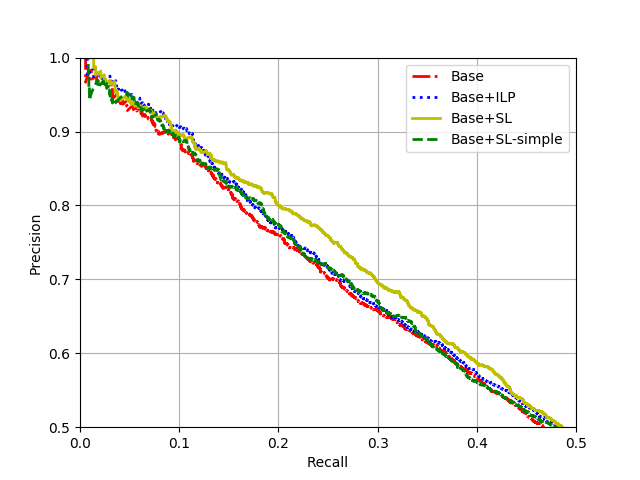
\includegraphics[width=7cm]{./result-figure/DBpedia-CNN-result.png}
		\caption{The English Dataset}
		\label{fig:dbpedia}
	\end{minipage}
	\begin{minipage}[t]{0.45\textwidth}
		\centering
		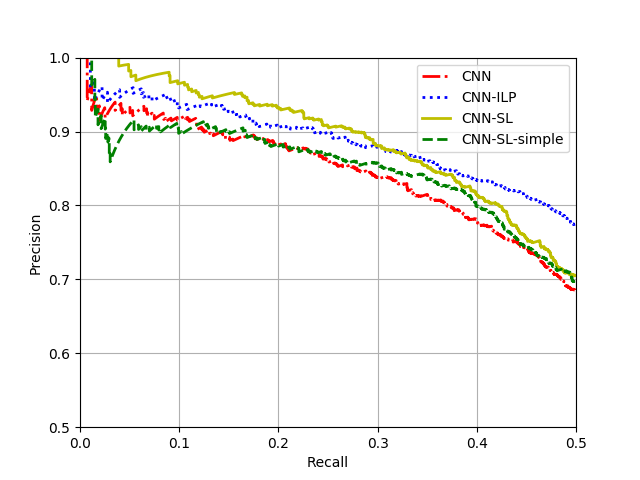
\includegraphics[width=7cm]{./result-figure/Chinese-CNN-result.png}
		\caption{The Chinese Dataset}
		\label{fig:chinese}
	\end{minipage}
\end{figure}

\paragraph{Compare with Base Model}
%Compare the semantic loss method and the base model (clear improvement).
As shown in Fig.~\ref{fig:dbpedia} and Fig.~\ref{fig:chinese}, by encouraging the base relation extractor to make predictions that are consistent to our constraints, our \SL method clearly improves the baseline relation extractor in both datasets.
%compared with the baseline, our framework performs consistently better in the DBpedia dataset and Chinese dataset. 
%In order to father demonstrate the semantic loss term helps to encode the constraints into relation extraction model, we count the tuple pairs that violates relation constraints introduced in Sec.~\ref{sec:constraints}, the results is show in Table ~\ref{table:violate-count}.
%IPE:  473.0 WPC:  440.0 CPNI:  273.0 CNN_C:  2123.0 SL_C:  2209.0

%In order to study how our framework improves the performances on the DBpedia dataset and the Chinese dataset, we further dig into the predictions of Base Model and SL Model, we find that our SL model corrects the Base Model's predictions to satisfy the constraints.
Take $<$\emph{Center For Responsible Lending, North Carolina}$>$ and $<$\emph{Meredith College, North Carolina}$>$ as an example.
\base outputs relations \emph{Location} and \emph{CoachedTeam} for these two entity pairs, and our \SL model predicts \emph{Location} and \emph{State} instead.
Note that \emph{Location} requires its subject to be a \underline{place}, and \emph{CoachedTeam} expects its subject to be a \underline{team}, so there exists a conflict between the two predictions.
\base confuses \emph{CoachedTeam} with \emph{State} since many team names are the same as their state names, and these two relations sometimes share similar expressions in the contexts. 
However, with the help of relation constraints during training, our semantic loss term identifies the conflict and thus encourages the base extractor to focus more on the textual clues about relation \emph{CoachedTeam}.
%and our SL Model eliminates the conflict through automatically learning constrain knowledge when training. 
%28 8 28 45 
\iffalse
\begin{table}
	\centering  
	\scriptsize  
	\caption{violate count}  
	\begin{tabular}{|c|c|c|c|c|}  
		\hline  
		 &Model&Type Violates&Cardinality Violates&Total\\  
		\hline 
		\multirow{2}*{DBpedia} & CNN & - & - & -\\
		~ & CNN-SL & - & - & -\\
		\hline 
		\multirow{2}*{Chinese} & CNN & - & - & -\\
		~ & CNN-SL & - & - & -\\ 
		\hline   
	\end{tabular} 
	
	\label{table:violate-count}  
\end{table}
\fi
\iffalse
\begin{figure}
	\centering
	\includegraphics[width=.4\textwidth]{./result-figure/CNN0-1.png}
	\caption{The DBpedia Dataset}
\end{figure}
\fi


\paragraph{Compare with ILP Method}
%Compare the semantic loss method and ILP.
%NOTE: clw also use cardinality constraints
%We use the same constraints information as the \ILP method of \cite{chen2014encoding}, and Figure ~\ref{fig:dbpedia} and Figure ~\ref{fig:chinese} shows that our SL method delivers superior performance compared to \ILP method in both DBpedia dataset and Chinese dataset.
As shown in Fig.~\ref{fig:dbpedia}, in the English dataset, \SL performs generally better than \ILP.
We think the superior performance comes from the fact that \SL functions during training and \ILP only acts as a post-processor.
Therefore, \SL can encourage the base model to find more textual clues when detecting conflicts, while \ILP can only find the most probable relation assignment that satisfies the constraints based on the output scores of the base model, which will possibly drop some high-score predictions and thus still leave the correct relation with a low score.

As for the Chinese dataset, based on the same reason, as shown in Fig.~\ref{fig:chinese}, we can see that \SL performs better in the high precision region.
%which is also caused by the fact that \ILP tend to leave the predictions corrected by the constraints with low scores.
However, we find that the constraints in Chinese are more effective than that in the English dataset, which leads to more corrections of the \ILP method.
Therefore, since \ILP tend to leave the predictions corrected by the constraints with low scores, a large fraction of the correct predictions gather around the low score region, which leads to higher precision of the \ILP curve in the high recall region.


%For DBpedia dataset, our method's performance is over \ILP method almost on all precision point. We think this is mainly because \ILP is a post-processing method which choose the most possible prediction that satisfy the constraints from the top three candidate results for every entity pairs, and this would drop some high score predictions, so for the high precision point, our SL method have better performance for both DBpedia dataset and Chinese Dataset. We also find that when recall in (0.3, 0.5), the \ILP is better than our SL method for Chinese Dataset, we think this is because adding constraints for Chinese dataset is much better than DBpedia dataset, the \ILP would drop more high score predictions and the right prediction corrected by \ILP is more likely appear at recall range (0.3, 0.5).


%and Fig.~\ref{fig:chinese}, when using the same constraints and base model, our \SL method is competitive to \ILP, and sometimes even performs better.

Note that, in practice, since we often require high-confidence extraction results, the performance of the high-precision region of the PR curve is more important than the low-precision one.
Further, recall that different from \ILP, \SL does not introduce extra cost during prediction.
These experiments indicate that our \SL method is more effective than \ILP in practice.
% the performance of high precision in PR curve is more important that the low precision, so totally our SL model gets superior performance than \ILP.
\paragraph{Compare with Simplified Semantic Loss}
%Compare the semantic loss method and the simplified semantic loss.
%Both on PR-curve, and on time.
%To reduce the time cost brought by semantic loss, as described in Sec.~\ref{Sec:simple_SL}, we simplify the calculation of our loss term by only using a subset of relation assignments.
%choosing some constraints from C in ~\ref{seq:semantic_loss} as new $\bm{C'}$, the $ \bm{C'} $ includes one most related constraint with the gold information of tuple pairs and 5 random sampling constraints, then we get the simplified semantic loss $ L^{s}_{simple}(\bm{C'}, \bm{p}) $ as follows:

%\begin{equation}
%\label{seq:semantic_loss_simple}
%L^{s}_{simple}(\bm{C'}, \bm{p}) = -log\sum\limits_{\bm x\models\bm{C'}}\prod\limits_{i:\bm x\models X_i}p_i\prod\limits_{i:\bm x\models \neg X_i}(1-p_i)
%\end{equation}

We also show the performance of our simplified semantic loss in Fig.~\ref{fig:dbpedia} and Fig.~\ref{fig:chinese} (\SLsimple).
We can see that, while inferior to \SL, \SLsimple also improves \base by a clear margin, and it is also comparable to \ILP in the English dataset.
In our experiments, compared to the original \SL method, \SLsimple reduces the extra training time introduced by calculating the semantic loss by 7 times in the English dataset, and 3 times in the Chinese dataset, which has less constraints than those in the English dataset.
%And both in DBpedia dataset and Chinese dataset the simplified semantic loss have improvement over Base Model, especially in DBpedia, it has comparable result with \ILP.
This indicates that \SLsimple acts as a good balance of the trade-off between extraction quality and extra training time.


